\chapter{Metodología}

Este capítulo trata de cubrir diversas rúbricas fundamentales para la evaluación del trabajo. Se abordarán las herramientas y metodologías empleadas para garantizar la calidad del código y la documentación, manteniendo altos estándares técnicos y de presentación. Finalmente, se describirá cómo se han implementado un enfoque ágil para adaptarse a los cambios y necesidades del cliente, demostrando la capacidad del proyecto para responder a imprevistos y nuevos requerimientos de manera eficaz.

\section{Enfoque ágil}

El proyecto seguirá las prácticas y principios del enfoque ágil, que se fundamenta en los 17 principios delineados en \href{https://agilemanifesto.org/iso/es/manifesto.html}{el manifiesto ágil}. Ágil no es una metodología ni un marco de trabajo, sino una mentalidad que permite a las organizaciones ser más receptivas al cambio. Estos principios están diseñados para asegurar la satisfacción del cliente a través de la entrega temprana y continua de valor, con un fuerte enfoque en la excelencia técnica, el buen diseño, la planificación y la simplicidad.

Estos principios no son solo una referencia teórica, sino que se han aplicado con éxito en proyectos reales y actuales, de acuerdo con~\cite{berlas2024software}. Este informe presenta una revisión completa de la investigación publicada sobre las métricas de software en el desarrollo ágil y resalta su efectividad en diversos contextos, incluyendo pequeñas y medianas empresas.

\begin{itemize}
    \item \textbf{¿Se están usando enfoques ágiles?} El informe indica que los enfoques ágiles son ampliamente utilizados en la industria del software, permitiendo a los equipos de desarrollo trabajar iterativamente y responder rápidamente a las necesidades del cliente.
    \item \textbf{¿Esto verdaderamente funciona?} Según el informe, los enfoques ágiles han demostrado ser eficaces en diversos tipos de proyectos a cualquier escala proporcionando beneficios como la reducción del tiempo de comercialización, mayor satisfacción del cliente y disminución de los costos de desarrollo.
\end{itemize}

\section{Entrega y calidad continua}

Para asegurar la calidad del proyecto y la entrega continua, se han empleado una serie de herramientas y metodologías que se han integrado en el flujo de trabajo tanto local como remoto.

La documentación del proyecto es una de las partes más importantes (junto con el código) del trabajo de fin de grado si no la que más por lo que se ha de poner especial atención en que esta sea de calidad y cumpla con los requisitos establecidos por tutor y tribunal. Para dar cuenta de esto, la memoria se ha elaborado en \href{https://www.latex-project.org/}{\LaTeX{}} que es un sistema de composición tipográfica de alta calidad; este incluye funciones diseñadas para la producción de documentación técnica y científica además de estar disponible como software libre.

\subsection{Flujo de trabajo local}

Para complementar, comprobar y mejorar la calidad de la documentación se han usado una serie de herramientas que se han integrado en el flujo de trabajo local tanto con extensiones de (\href{https://code.visualstudio.com/}{\textit{Visual Studio Code}}) como con herramientas ejecutadas en la línea de comandos.

Más adelante se detallarán las herramientas utilizadas y el proceso de selección de las mismas.

\subsection{Flujo de trabajo remoto}

Estos flujos se realizan en \textit{GitHub} implementando uno específico para la memoria. Este flujo de trabajo se activa en cada \textit{push} y se encarga de ejecutar verificaciones gramaticales y ortográficas con \href{https://github.com/sylvainhalle/textidote}{\textit{TeXtidote}}~\ref{sec:textidote} de la cual se sube un informe y si pasa estas verificaciones de forma satisfactoria se sube la memoria compilada en formato PDF a modo de artefacto. Este flujo de trabajo remoto junto con el local garantizan la calidad de la documentación.

Ese artefacto generado tras acabar cada \textit{milestone} o hito podría ser perfectamente entregable a un cliente final a modo de entrega continua para que vea el progreso del proyecto. A mayores, hacemos referencia al tercer principio del \href{https://agilemanifesto.org/iso/es/principles.html}{manifiesto ágil} que dice: \textit{``Entregar software funcional frecuentemente, entre dos semanas y dos meses, con preferencia al periodo de tiempo más corto''}. Además, los flujos de trabajo remotos (en \textit{GitHub}) y locales promueven el noveno principio que hace referencia a la atención continua a la excelencia técnica y el buen diseño.

\section{Herramientas y metodologías utilizadas}

En esta sección se documentarán las metodologías empleadas para el seguimiento del desarrollo del proyecto. Al aplicar estas metodologías se ha conseguido una mayor eficiencia en la gestión del tiempo y de los recursos, así como una mayor calidad en la documentación y en el código fuente. Además, se explicarán las herramientas utilizadas para el control de versiones y el alojamiento del repositorio remoto del proyecto.

\subsection{\textit{Git y GitHub}: control de versiones y colaboración}

Para el control de versiones se ha empleado \textit{git} que es un sistema de control de versiones que permite llevar un control de los cambios en el código fuente.

Para la colaboración y hospedaje del código fuente se ha hecho en \textit{GitHub}, una plataforma que permite alojar proyectos de \textit{software} y colaborar en ellos. En \textit{GitHub} tenemos diferentes funcionalidades que han sido de ayuda para el desarrollo del proyecto.

\textbf{El repositorio del proyecto se puede encontrar en la siguiente dirección: \url{https://github.com/danigonzser/proyecto-tfg}.}

La transparencia y accesibilidad de GitHub facilitan la comunicación constante y la colaboración del equipo, apoyando los principios ágiles de la colaboración diaria entre desarrolladores y clientes, y de la construcción de proyectos en torno a individuos motivados.

En GitHub se integran diferentes herramientas que permiten llevar un control del desarrollo del proyecto. A continuación, se describen algunas de las funcionalidades más importantes.

\subsection{Pull requests}

Los pull requests son una manera de proponer cambios en el código fuente sin que estos se apliquen directamente al código fuente o rama principal sin una aprobación previa. Esta metodología garantiza que los cambios mantengan la excelencia técnica y calidad del proyecto apoyando al noveno principio del manifiesto ágil.

Para proteger la rama principal o \textit{master} de cambios no deseados se han configurado una serie de reglas que impiden la integración de cambios a menos que:

\begin{itemize}
    \item Los tests deben de haberse realizado de manera exitosa.
    \item Que la rama esté actualizada.
    \item Que las conversaciones hayan sido resueltas.
\end{itemize}

A continuación se muestra una captura de pantalla de la lista de \textit{pull requests} del proyecto hasta el momento.

\begin{figure}[H]
    \caption{Captura de pantalla del listado de \textit{pull requests} del repositorio del proyecto de \textit{GitHub}.}
    \centering
    \vspace*{0.5cm}
    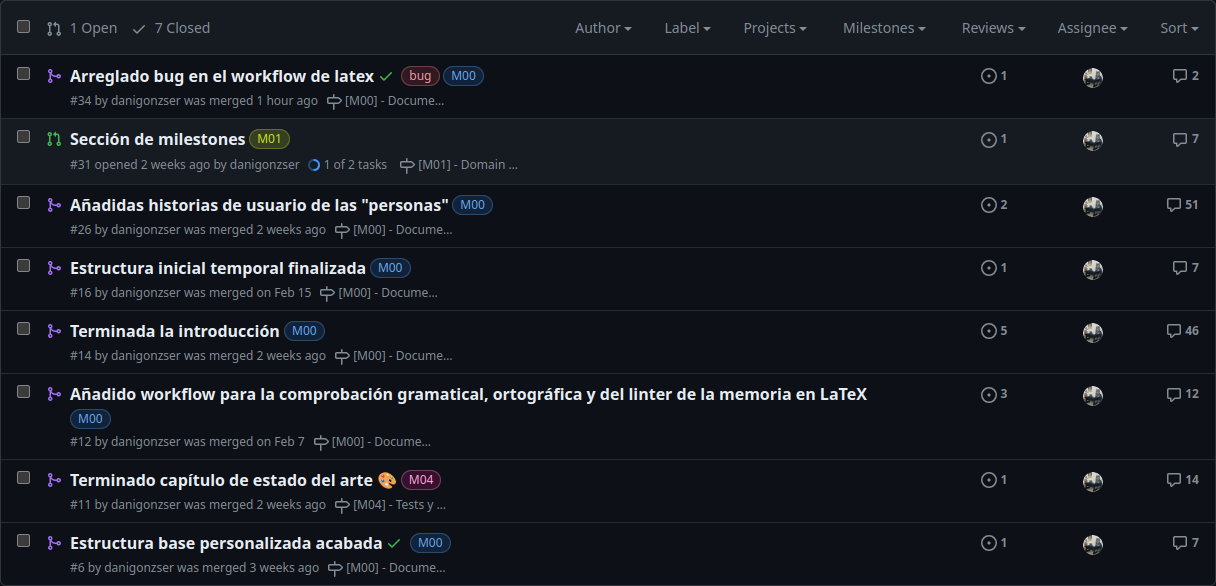
\includegraphics[scale=0.2]{figuras/listado_pull_requests_github.png}
\end{figure}

En la figura se puede apreciar que se han abierto 8 \textit{pull requests} hasta el momento. Los que están en color morado son los \textit{pull requests} que ya han sido integrados en la rama principal y el que está en color verde es el que todavía no está integrado.

\begin{figure}[H]
    \caption{Captura de pantalla del contenido de una \textit{pull request}.}
    \centering
    \vspace*{0.5cm}
    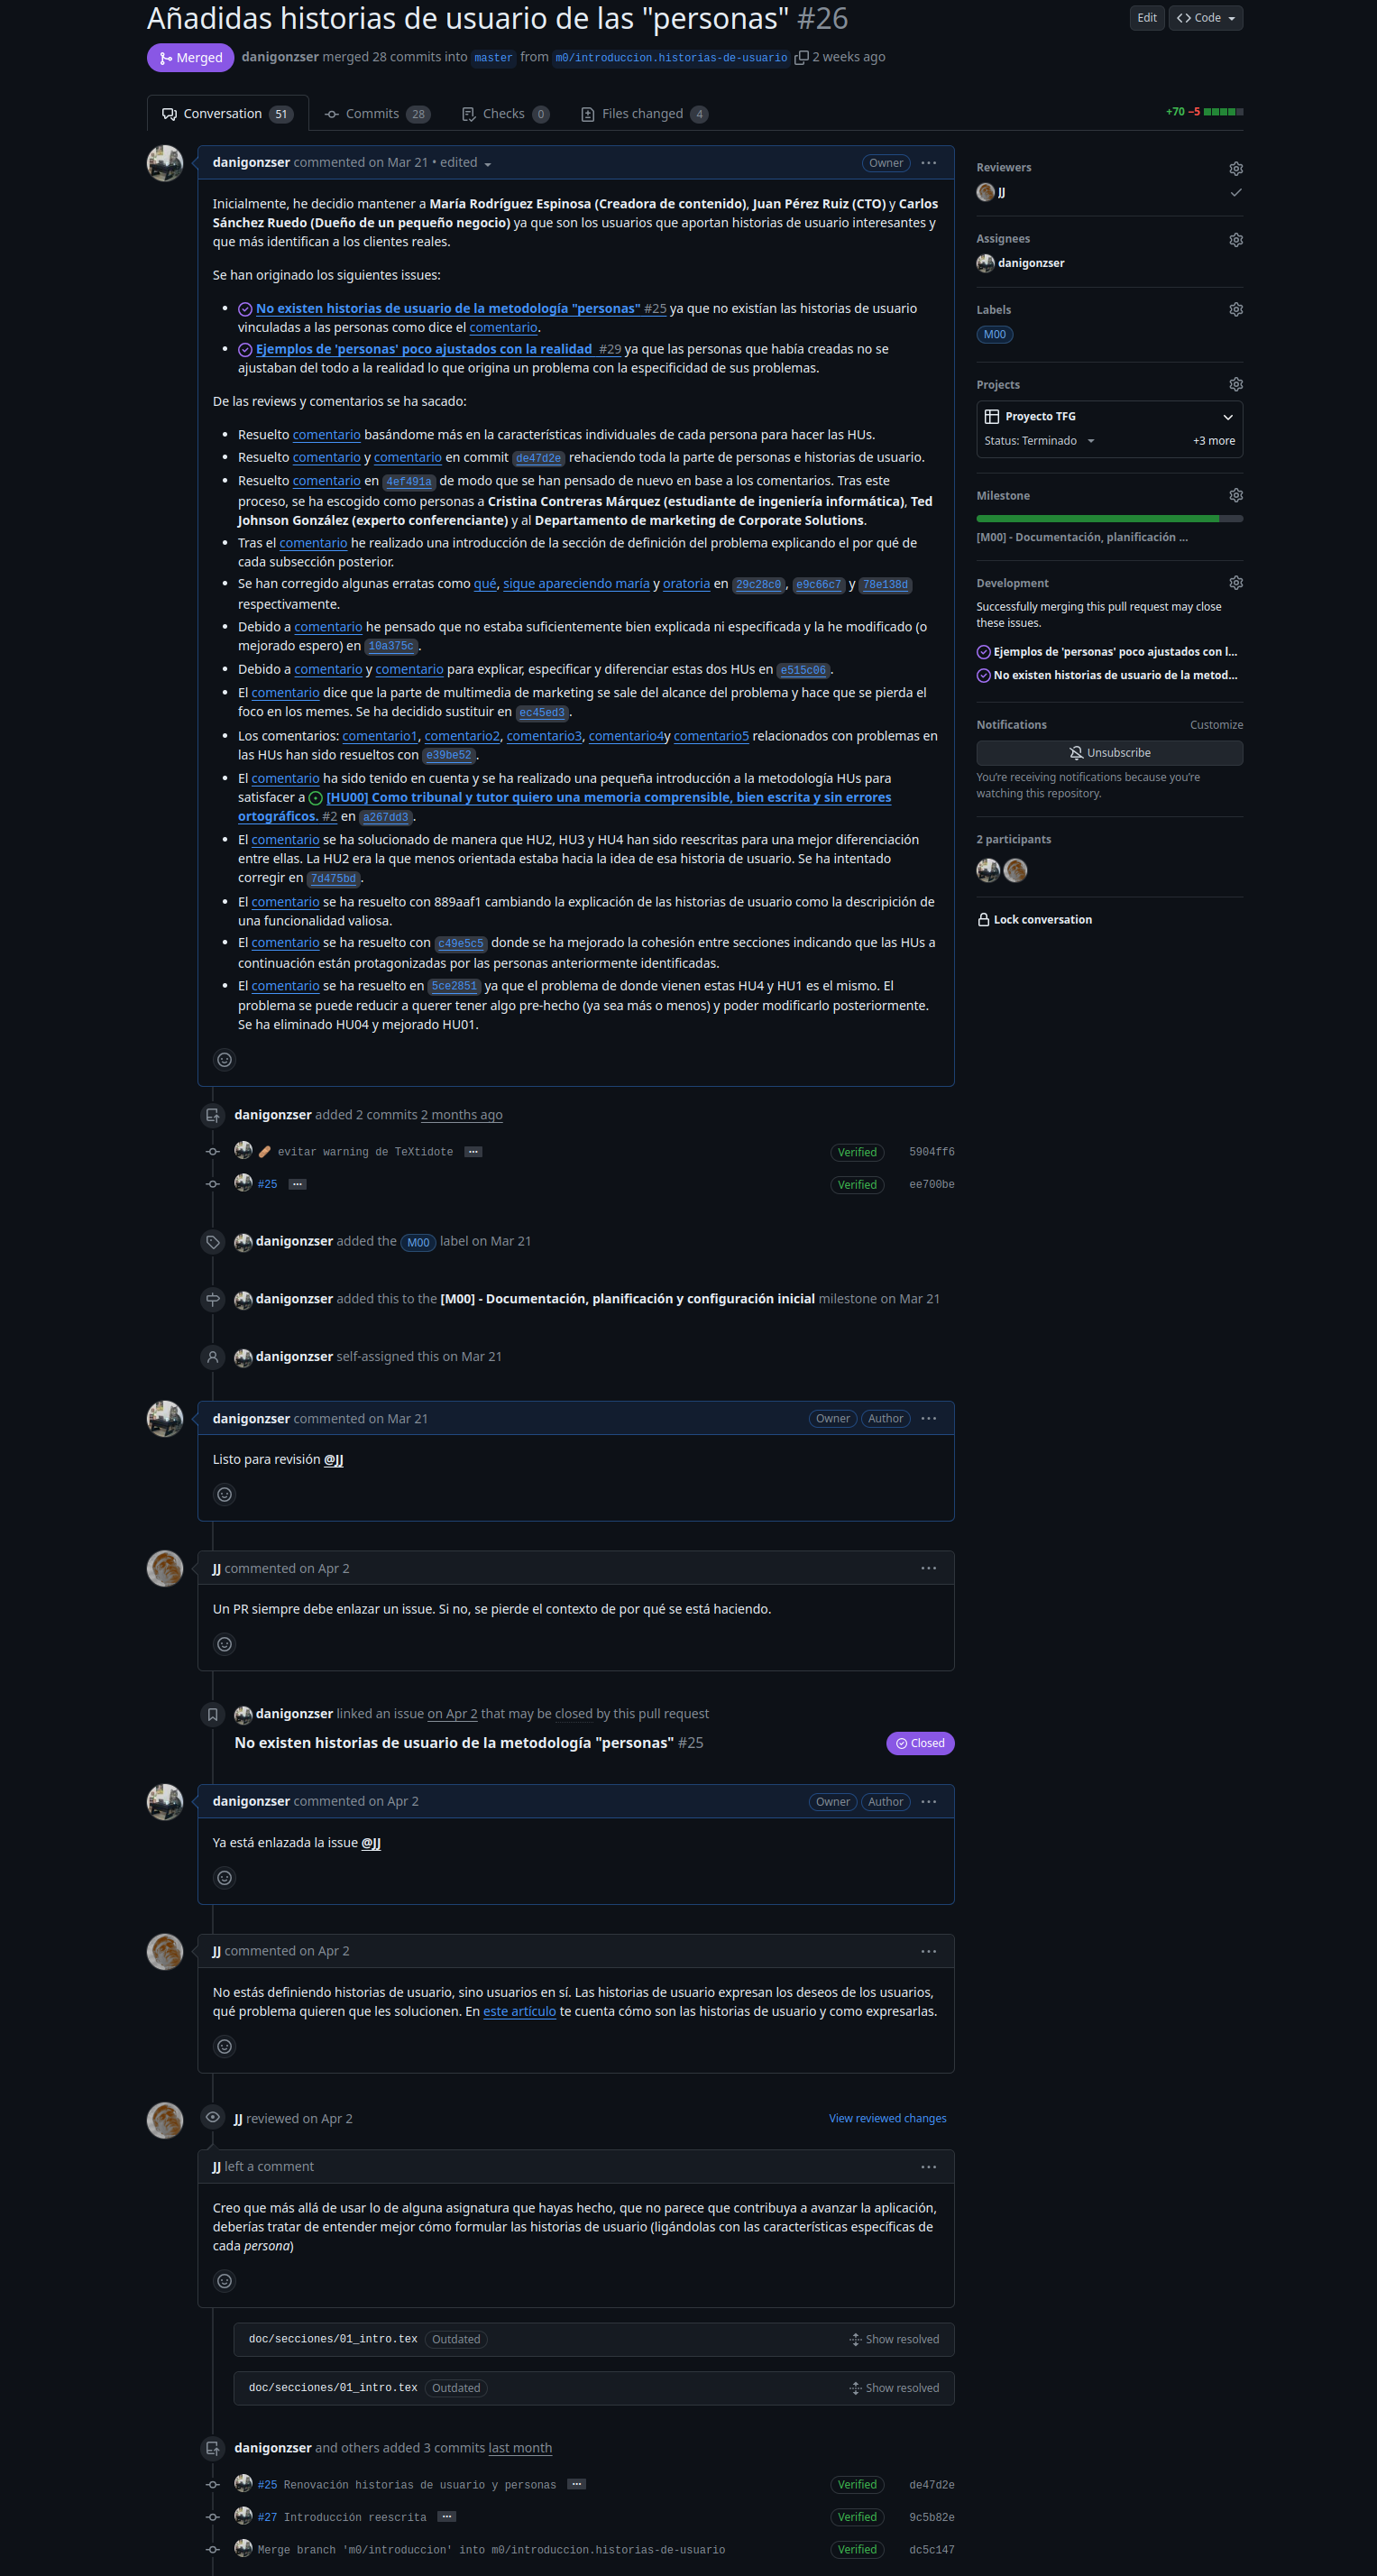
\includegraphics[scale=0.1]{figuras/pull_request_github.png}\label{fig:contenido_pull_request}
\end{figure}

Como se puede ver en la figura~\ref{fig:contenido_pull_request} el estado de la \textit{pull request} es \textit{merged} lo que significa que ya ha sido integrado en la rama principal. Más abajo se puede ver el cuerpo de la misma donde residen todas las \textit{issues} que han sido creadas y consecuentemente resueltas con esta \textit{pull request}. Más abajo se puede ver el historial de commits y de conversaciones que se han ido originando a lo largo de la resolución. Al final de la imagen es donde podemos ver esas conversaciones que deben ser resueltas antes de integrar los cambios en la rama principal. Finalmente, a la derecha se muestran detalles como el revisor, el asignado, las etiquetas, el proyecto al que pertenece, el \textit{milestone} y las \textit{issues} relacionadas.

\subsection{\textit{Projects}: tablero kanban}

La funcionalidad de projects de \textit{GitHub} se ha utilizado para llevar un control de la evolución y progreso de los \textit{issues} y \textit{pull requests}. Se ha implementado un tablero \textit{kanban} como se puede ver en la imagen~\ref{fig:tablero_kanban} que permite ver de un vistazo el estado de los \textit{issues} y \textit{pull requests}. Esto es muy útil para saber si se progresa, cómo se están resolviendo los problemas y si se está cumpliendo con los objetivos marcados. Además, está relacionado con los principios ágiles al promover la autoorganización, entrega frecuente y temprana y atención continua.

\begin{figure}[H]
    \caption{Captura de pantalla del tablero \textit{kanban} en la sección de \textit{projects} de \textit{GitHub}.}
    \centering
    \vspace*{0.5cm}
    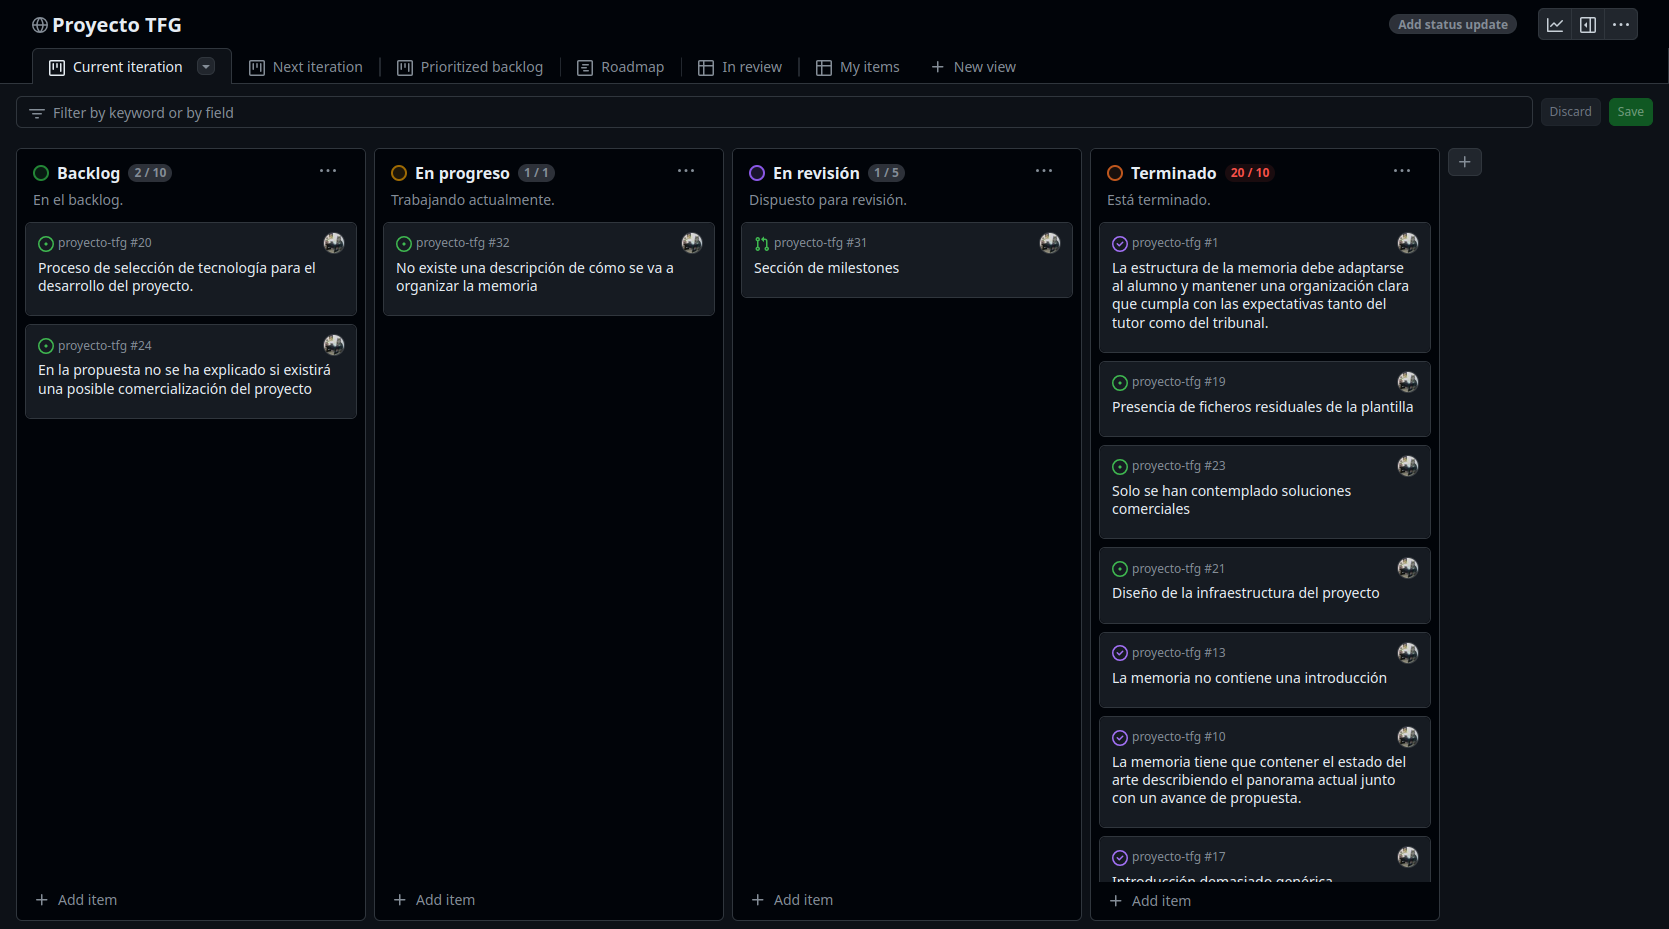
\includegraphics[scale=0.2]{figuras/projects_github.png}\label{fig:tablero_kanban}
\end{figure}

\section{Memoria}

A la hora de seleccionar la opción más adecuada para cada aspecto que se incluirá en la memoria, se empleó un riguroso proceso de selección. Para ello fue necesario articular claramente los fundamentos de la decisión, esbozar los criterios de búsqueda, especificar los requisitos de la herramienta y justificar detalladamente la elección final.

\subsection{Corrector ortográfico y gramatical}

La corrección ortográfica y gramatical es un aspecto fundamental en la redacción de cualquier documento. Este documento no es una excepción, por lo que se han empleado una serie de herramientas para garantizar la calidad de la redacción. Como hemos comentado previamente vamos a explicar el proceso de selección para satisfacer este aspecto.

\subsubsection{Marco de selección}

El uso de un corrector ortográfico y gramatical en un texto de alta calidad es esencial para lograr claridad y profesionalismo en la comunicación escrita. No se trata solo de evitar errores ortográficos, sino de pulir cada detalle para que el mensaje transmita cuidado y atención. Un texto bien corregido además de comunicar información, también crea una conexión efectiva con el lector. Los errores pueden distraer y restar valor al trabajo, afectando la credibilidad, calidad y dedicación del autor por parte del lector. Por ello, es crucial evitar estos errores para asegurar que el mensaje llegue con la fuerza y claridad deseadas.

Es evidente que la corrección automática no es infalible, por lo que no se le puede delegar toda la responsabilidad. Es fundamental que el autor revise el texto para asegurar que la comprobación sea precisa y no se hayan pasado por alto errores. Esta sirve como un apoyo, pero no sustituye la revisión manual.

\subsubsection{Criterios de búsqueda}

En esta sección, se detallarán los criterios que guiarán la búsqueda de posibles soluciones y herramientas. Estos criterios reflejan tanto las necesidades técnicas como los objetivos estratégicos del proyecto, proporcionando una base sólida para la toma de decisiones. 

\begin{itemize}
    \item Debe ser compatible con~\LaTeX{} de forma nativa, ya que no se ha encontrado ninguna herramienta que elimine por completo código \LaTeX{} que sea fiable y estable.
    \item Debe contemplar el diccionario español.
\end{itemize}

\subsubsection{Criterios de selección}

En esta sección, se detallarán los criterios de selección que se utilizarán para evaluar las posibles soluciones y herramientas.

\begin{itemize}
    \item \textbf{Actualidad:} La herramienta debe ser actualizada regularmente para garantizar la incorporación de nuevas funcionalidades, diccionarios y reglas.
    \item \textbf{Exactitud:} La herramienta debe ser precisa.
    \item \textbf{Fiabilidad:} La herramienta debe ser estable y no presentar fallos o errores en su funcionamiento.
    \item \textbf{Facilidad de uso:} La herramienta debe ser fácil de usar e intuitiva para el usuario.
    \item \textbf{Integración local:} La herramienta debe poder integrarse en el flujo de trabajo de \textit{Visual Studio Code}.
    \item \textbf{Integración remota:} La herramienta debe poder integrarse en el flujo de trabajo de \textit{GitHub Actions}.
    \item \textbf{Rapidez:} Se valora que la herramienta sea rápida.
    \item \textbf{Soporte:} La herramienta debe contar con un soporte técnico o de la comunidad.
    \item \textbf{Retroalimentación:} La herramienta debe proporcionar retroalimentación al usuario sobre los errores y sugerencias.
\end{itemize}

\subsubsection{Herramientas seleccionadas}

Una vez establecidos los criterios de búsqueda y de selección se va a proceder a listar las herramientas o soluciones destacadas. Las características en referencia a los criterios de selección se categorizan en \textit{mal} (\mal), \textit{regular} (\regular), \textit{bien} (\bien) y \textit{excelente} (\esp) dependiendo de su cumplimiento con el criterio.

\subsubsection{\href{https://github.com/sylvainhalle/textidote}{\textit{TeXtidote}}}~\label{sec:textidote}

\textit{TeXtidote} es una herramienta de línea de comandos que se puede utilizar para comprobar la gramática y la ortografía de documentos escritos en LaTeX. \textit{TeXtidote} realiza una serie de comprobaciones para garantizar la coherencia y calidad del documento. Además, puede eliminar cualquier formato del archivo y enviarlo a la librería de \textit{LanguageTool} interna. Una de sus características distintivas es su capacidad para controlar la posición relativa de las palabras entre el texto original y el texto corregido. Esto permite que los mensajes de error se sitúen en la ubicación exacta del mismo.

En nuestro caso, se ha empleado para ejecutarlo de forma local, para la integración continua de la memoria en el repositorio remoto de \textit{GitHub}. Para ello, se ha configurado un \textit{workflow} de \textit{GitHub Actions} que se encarga de ejecutar \textit{TeXtidote} en la memoria y de subir los resultados a la rama principal.

\begin{itemize}
    \item[\bien] \textbf{Actualidad:}  Se han hecho cambios en la rama principal del repositorio hace tres meses.
    \item[\bien] \textbf{Exactitud:} Es bastante preciso en las correcciones, ya que utiliza una instancia de \textit{LanguageTool} interna.
    \item[\regular] \textbf{Fiabilidad:} Está especializado en~\LaTeX{} aunque presenta problemas a la hora de omitir algún macro o comando interno.
    \item[\esp] \textbf{Facilidad de uso:} Aunque la herramienta deba ejecutarse por línea de comandos y debamos configurarla para que funcione correctamente, la facilidad de uso es lo mejor que tiene, ya que automáticamente tras una orden puede llegar a analizar toda la memoria.
    \item[\mal] \textbf{Integración local:} No se integra directamente en \textit{Visual Studio Code}, puesto que no existe una extensión.
    \item[\bien] \textbf{Integración remota:} Existe una \textit{GitHub action} que se encarga de ejecutar \textit{TeXtidote} en la memoria y poder generar artefactos con los resultados. 
    \item[\regular] \textbf{Rapidez:} Puede llegar a ser bastante lenta aún en documentos pequeños.
    \item[\regular] \textbf{Soporte:} Ya que no sufre actualizaciones el soporte es bastante limitado aunque al ser código abierto existe una comunidad detrás.
    \item[\bien] \textbf{Retroalimentación:} Lo mejor que tiene es la retroalimentación que proporciona al usuario en forma de página HTML con los errores y sugerencias por fichero.
\end{itemize}

\subsubsection{\href{https://github.com/languagetool-org/languagetool}{\textit{LanguageTool}}}\label{sec:languagetool}

\textit{LanguageTool} es un corrector gramático y estilístico de código abierto que se puede utilizar para comprobar la gramática y la ortografía en varios idiomas. Tiene varias opciones para integrar: mediante una biblioteca de Java, una herramienta de línea de comandos, una extensión de navegador o un servidor web.

\begin{itemize}
    \item[\bien] \textbf{Actualidad:}  Al estar en producción y tras una empresa el código se actualiza regularmente.
    \item[\bien] \textbf{Exactitud:} Es precisa en las correcciones, ya que sufre actualizaciones constantemente añadiendo palabras y reglas.
    \item[\bien] \textbf{Fiabilidad:} Es estable en su funcionamiento.
    \item[\regular] \textbf{Facilidad de uso:} Si se quiere experimentar en pleno funcionamiento (y gratis) se debe levantar un servidor local al cual hacer peticiones. No tiene integración nativa.
    \item[\esp] \textbf{Integración local:} La extensión \href{https://github.com/valentjn/vscode-ltex}{\textit{LTeX LanguageTool grammar/spell checking}} permite una integración total en local desde \textit{Visual Studio Code}, tiene la opción de poder configurar un servidor local de \textit{LanguageTool} para mejorar las comprobaciones aunque por defecto se haga a través de una versión interna de \textit{LanguageTool}.
    \item[\mal] \textbf{Integración remota:} No existe una integración en \textit{GitHub Actions} incluso sería bastante complicado de implementar debido a la necesidad de un servidor local.
    \item[\regular] \textbf{Rapidez:} Más rápida que \textit{TeXtidote} aunque puede llegar a ser bastante lenta en documentos muy extensos.
    \item[\bien] \textbf{Soporte:} Tiene un soporte bastante extenso al ser una empresa la que lo mantiene.
    \item[\bien] \textbf{Retroalimentación:} Con la extensión, la retroalimentación que proporciona el usuario es buena, ya que se puede ver en tiempo real los fallos y se ofrecen sugerencias.
\end{itemize}

\subsubsection{Opciones descartadas en el proceso de búsqueda}

\begin{itemize}
    \item \textbf{\href{https://www.grammarly.com/}{Grammarly}:} Aunque es una de las herramientas más conocidas y utilizadas, no se ha seleccionado debido a que no es compatible con \LaTeX{} por lo que se tendría que utilizar con una herramienta que elimine este formato.
    \item \textbf{\href{http://aspell.net/}{GNU Aspell}:} Es una de las herramientas más veteranas aunque ha sido descartada debido a que solo hace revisiones ortográficas.
    \item \textbf{\href{https://www.cs.hmc.edu/~geoff/ispell.html}{Ispell}:} Ha sido descartada por la misma razón que la anterior.
\end{itemize}

\subsubsection{Conclusiones}

Tras el análisis, se ha decidido que, con respecto al flujo de trabajo local tanto \textit{TeXtidote} a través de la línea de comandos como la extensión para el editor de código de \textit{LanguageTool} se van a emplear para la corrección ortográfica y gramatical de la memoria. En nuestro caso y para mejorar las comprobaciones se ha configurado para que trabaje a través de peticiones \textit{HTTP} a un contenedor de \textit{Docker} con la imagen \href{https://hub.docker.com/r/erikvl87/languagetool}{erikvl87/languagetool} a modo de servidor. En adición, se ha añadido un conjunto de datos de \href{https://es.wikipedia.org/wiki/N-grama}{n-gramas} para \href{https://dev.languagetool.org/finding-errors-using-n-gram-data}{detectar errores} con palabras que suelen confundirse.

En la parte de integración continua y/o flujo de trabajo remoto debido a su facilidad de uso, a su integración con \LaTeX{} y a su retroalimentación basado en informes \textit{HTML} se ha decidido usar \href{https://github.com/marketplace/actions/textidote-action}{TeXtidote Action}.

\section{Organización de código \LaTeX{}}

En esta sección se documentarán las herramientas empleadas en las que me he basado a la hora de organizar y/o planificar el proyecto.

\subsection{Extensión de \textit{Visual Studio Code}: \textit{LaTeX Workshop}}

LaTeX Workshop es una extensión para Visual Studio Code, cuyo objetivo es proporcionar funciones básicas para la composición tipográfica LaTeX con Visual Studio Code. Esta extensión proporciona una serie de características que facilitan la escritura de documentos en LaTeX como la previsualización en tiempo real, la compilación del documento, la visualización de errores y advertencias.

A mayores, esta extensión me ha permitido elegir la receta de compilación que se va a utilizar, la cual se ha configurado para que se compile la memoria junto con la bibliografía.

\begin{figure}[H]
    \caption{Captura de pantalla de \textit{Visual Studio Code} con la extensión \textit{LaTeX Workshop} activada.}
    \centering
    \vspace*{0.5cm}
    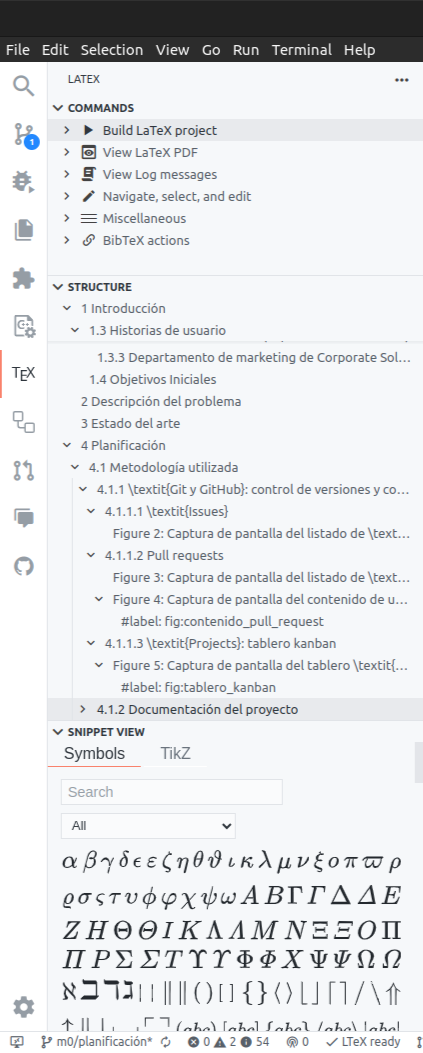
\includegraphics[scale=0.2]{figuras/latex_workshop_extension.png}\label{fig:latex_workshop_extension}
\end{figure}

\subsection{Extensión de \textit{Visual Studio Code}: \href{https://github.com/valentjn/vscode-ltex}{\textit{LTeX LanguageTool grammar/spell checking}}}

La extensión \( LT_E X \) permite comprobar la gramática y la ortografía de varios lenguajes de marcado en \textit{Visual Studio Code} mediante \textit{LanguageTool}.

Esta extensión suele trabajar de forma offline teniendo una instancia local de \textit{LanguageTool}, pero en nuestro caso se ha configurado para que trabaje con una instancia remota de \textit{LanguageTool} que se ejecuta en un contenedor de \textit{Docker} como hemos dicho anteriormente.

\begin{quote}
    \textbf{Nota}: El estilo del código \LaTeX{} se ha configurado mediante esta extensión para ser verificado cada vez que se guarda con \href{https://www.nongnu.org/chktex/}{ChkTeX} y \href{https://ctan.org/pkg/lacheck}{LaCheck}. Aunque esta característica no es tan crucial como en otros lenguajes de programación, puede ayudar a detectar errores comunes en la redacción de documentos. Por estos motivos, y dado que la integración con esta extensión era muy sencilla, no se ha llevado a cabo un proceso de selección ni una verificación en el flujo de trabajo remoto.
\end{quote}